\section{Verwendete Werkzeuge}
\label{sec:Werkzeuge}
BEREITS BEARBEITET!\\
Im Folgenden werden die Hardware und Software vorgestellt, welche die Autoren zum Erstellen dieser Arbeit und vor allem zur Entwicklung der App verwendet haben. Es wurden ausschliesslich Open-Source-Programme eingesetzt.\\
Hier benutzte Beschreibungen k�nne von Website (offizielle Site der Software, Wikipedia...) �bernommen sein. Dieser Abschnitt dient zur Information f�r die verwendeten Werkzeuge.
\subsection{Software}
\begin{itemize}


\item \textbf{\LaTeX} \\
Diese Arbeit wurde mit {\LaTeX} geschrieben. Als Distribution und Editor wurde auf dem Mac OS Mountain Lion TexShop verwendet, auf Basis von Linux ????????????. \\
Websites: \url{http://pages.uoregon.edu/koch/texshop/}
\end{itemize}

\subsection{Hardware}
ALLES HIER IST AKUTELL\\
Ausser die Sch*** Tabelle, die sich nicht formatieren lassen m�chte...\\
\begin{itemize}

\item \textbf{Galaxy Nexus} \\
Auf diesem Smartphone l�uft das brandaktuelle Andoid OS 4.1.1 (Nelly Bean).\\
\begin{tabular}[t]{|l|l|c|} \hline
 \cellcolor{darkgrey} &  \cellcolor{darkgrey} & \\
\cellcolor{darkgrey} \multirow{-2}{3cm}{\textbf{Bezeichnung}} &
\cellcolor{darkgrey} \multirow{-2}{6cm}{\textbf{Version}} &  \\
model number & Galaxy Nexus & \\ \cline{1-2}
Android-Version & 4.1.1 (Jelly Bean) &\\ \cline{1-2}
Baseband-Version & I9250XXLF1 &\\   \cline{1-2}
Kernel-Version & 3.0.31-g6fb96c9 &\\  \cline{1-2}
Build number & JR003C.I9250XWLH2 & \\  \cline{1-2}
Screen Resolution & 1280 x 720 pixel & \\ \cline{1-2}
diagonal & 4.65 inch & \multirow{-8}{6cm}{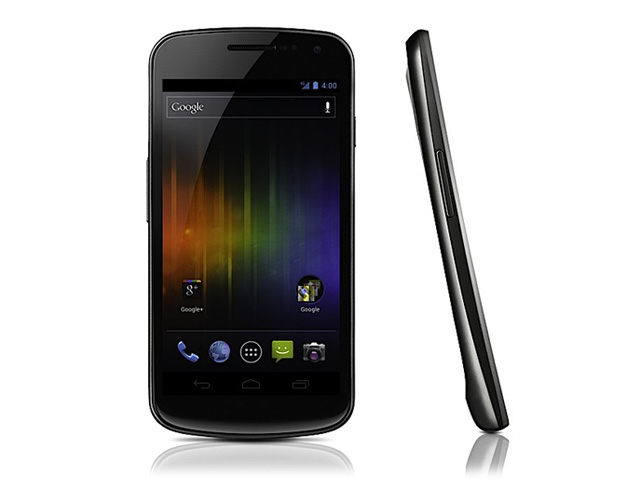
\includegraphics[width=6cm]{galaxynexus.png} }\\  \hline 
\end{tabular}\\



\item \textbf{Gr�enis Phone...} \\
\begin{tabular}[t]{|l|l|} \hline
 \rowcolor{darkgrey} &\\
\rowcolor{darkgrey}
\multirow{-2}{3cm}{\textbf{Bezeichnung}} &
\multirow{-2}{10cm}{\textbf{Version}} \\
model number & \\ \hline 
Android-Version & \\  \hline 
Baseband-Version &  \\  \hline 
Kernel-Version & \\  \hline 
Build number &  \\  \hline 
Screen Resolution &\\  \hline 
diagonal & \\  \hline 
\end{tabular}\\


\end{itemize}